\documentclass[,aspectratio=43]{beamer}

% Load theme ---------------------------------------------------------------------------------

\usetheme[progressdots,transitions,banner,logo]{ubd}

% Information for the title page -------------------------------------------------------------
\author{Haziq Jamil}

\title{Regression modelling using I-priors}

\title{Regression modelling using I-priors}

\subtitle{NUS Department of Statistics \& Data Science Seminar}

\institute{Mathematical Sciences, Faculty of Science, UBD\\
\url{https://haziqj.ml}}

\date{Wednesday, 16 November 2022}

% Font fix -----------------------------------------------------------------------------------
% \usepackage{ifxetex,ifluatex}
% \ifnum 0\ifxetex 1\fi\ifluatex 1\fi=0 % if pdftex
%   \usepackage[T1]{fontenc}
%   \usepackage[utf8]{inputenc}
%   \usepackage{textcomp} % provide euro and other symbols
% \else % if luatex or xetex
%   \usepackage{unicode-math}
%   \defaultfontfeatures{Scale=MatchLowercase}
%   \defaultfontfeatures[\rmfamily]{Ligatures=TeX,Scale=1}
% \fi

\usepackage{soul}
\makeatletter
\let\HL\hl
\renewcommand\hl{%
  \let\set@color\beamerorig@set@color
  \let\reset@color\beamerorig@reset@color
  \HL}
\makeatother
% https://tex.stackexchange.com/questions/460731/highlight-color-a-part-of-text-in-block-in-beamer
\newcommand{\hlc}[2][yellow]{{%
    \colorlet{foo}{#1}%
    \sethlcolor{foo}\hl{#2}}%
}
% https://tex.stackexchange.com/questions/352956/how-to-highlight-text-with-an-arbitrary-color

% knitr stuff --------------------------------------------------------------------------------
\usepackage{color}
\usepackage{fancyvrb}
\newcommand{\VerbBar}{|}
\newcommand{\VERB}{\Verb[commandchars=\\\{\}]}
\DefineVerbatimEnvironment{Highlighting}{Verbatim}{commandchars=\\\{\}}
% Add ',fontsize=\small' for more characters per line
\usepackage{framed}
\definecolor{shadecolor}{RGB}{248,248,248}
\newenvironment{Shaded}{\begin{snugshade}}{\end{snugshade}}
\newcommand{\AlertTok}[1]{\textcolor[rgb]{0.94,0.16,0.16}{#1}}
\newcommand{\AnnotationTok}[1]{\textcolor[rgb]{0.56,0.35,0.01}{\textbf{\textit{#1}}}}
\newcommand{\AttributeTok}[1]{\textcolor[rgb]{0.77,0.63,0.00}{#1}}
\newcommand{\BaseNTok}[1]{\textcolor[rgb]{0.00,0.00,0.81}{#1}}
\newcommand{\BuiltInTok}[1]{#1}
\newcommand{\CharTok}[1]{\textcolor[rgb]{0.31,0.60,0.02}{#1}}
\newcommand{\CommentTok}[1]{\textcolor[rgb]{0.56,0.35,0.01}{\textit{#1}}}
\newcommand{\CommentVarTok}[1]{\textcolor[rgb]{0.56,0.35,0.01}{\textbf{\textit{#1}}}}
\newcommand{\ConstantTok}[1]{\textcolor[rgb]{0.00,0.00,0.00}{#1}}
\newcommand{\ControlFlowTok}[1]{\textcolor[rgb]{0.13,0.29,0.53}{\textbf{#1}}}
\newcommand{\DataTypeTok}[1]{\textcolor[rgb]{0.13,0.29,0.53}{#1}}
\newcommand{\DecValTok}[1]{\textcolor[rgb]{0.00,0.00,0.81}{#1}}
\newcommand{\DocumentationTok}[1]{\textcolor[rgb]{0.56,0.35,0.01}{\textbf{\textit{#1}}}}
\newcommand{\ErrorTok}[1]{\textcolor[rgb]{0.64,0.00,0.00}{\textbf{#1}}}
\newcommand{\ExtensionTok}[1]{#1}
\newcommand{\FloatTok}[1]{\textcolor[rgb]{0.00,0.00,0.81}{#1}}
\newcommand{\FunctionTok}[1]{\textcolor[rgb]{0.00,0.00,0.00}{#1}}
\newcommand{\ImportTok}[1]{#1}
\newcommand{\InformationTok}[1]{\textcolor[rgb]{0.56,0.35,0.01}{\textbf{\textit{#1}}}}
\newcommand{\KeywordTok}[1]{\textcolor[rgb]{0.13,0.29,0.53}{\textbf{#1}}}
\newcommand{\NormalTok}[1]{#1}
\newcommand{\OperatorTok}[1]{\textcolor[rgb]{0.81,0.36,0.00}{\textbf{#1}}}
\newcommand{\OtherTok}[1]{\textcolor[rgb]{0.56,0.35,0.01}{#1}}
\newcommand{\PreprocessorTok}[1]{\textcolor[rgb]{0.56,0.35,0.01}{\textit{#1}}}
\newcommand{\RegionMarkerTok}[1]{#1}
\newcommand{\SpecialCharTok}[1]{\textcolor[rgb]{0.00,0.00,0.00}{#1}}
\newcommand{\SpecialStringTok}[1]{\textcolor[rgb]{0.31,0.60,0.02}{#1}}
\newcommand{\StringTok}[1]{\textcolor[rgb]{0.31,0.60,0.02}{#1}}
\newcommand{\VariableTok}[1]{\textcolor[rgb]{0.00,0.00,0.00}{#1}}
\newcommand{\VerbatimStringTok}[1]{\textcolor[rgb]{0.31,0.60,0.02}{#1}}
\newcommand{\WarningTok}[1]{\textcolor[rgb]{0.56,0.35,0.01}{\textbf{\textit{#1}}}}
\usepackage{graphicx,grffile}
\makeatletter
\def\maxwidth{\ifdim\Gin@nat@width>\linewidth\linewidth\else\Gin@nat@width\fi}
\def\maxheight{\ifdim\Gin@nat@height>\textheight\textheight\else\Gin@nat@height\fi}
\makeatother
% Scale images if necessary, so that they will not overflow the page
% margins by default, and it is still possible to overwrite the defaults
% using explicit options in \includegraphics[width, height, ...]{}
\setkeys{Gin}{width=\maxwidth,height=\maxheight,keepaspectratio}
% Set default figure placement to htbp
\makeatletter
\def\fps@figure{htbp}
\makeatother
\setlength{\emergencystretch}{3em} % prevent overfull lines
\providecommand{\tightlist}{%
  \setlength{\itemsep}{0pt}\setlength{\parskip}{0pt}}
\setcounter{secnumdepth}{-\maxdimen} % remove section numbering

% Packages -----------------------------------------------------------------------------------
% \setlength{\parskip}{1em}
\usepackage{tikz}
\usetikzlibrary{shapes.geometric,fit,arrows.meta}
\usepackage{xltabular}
\usepackage{longtable,booktabs,multirow,colortbl}
\usepackage{caption}
% Make caption package work with longtable
\makeatletter
\def\fnum@table{\tablename~\thetable}
\makeatother
\usepackage{lipsum}
\usepackage{csquotes}

% To use arabic -----------------------------------------------------------------------------
% WARNING: Using arabic script causes some issues with footnotes.
% Packages are not loaded by default

\usepackage{polyglossia}  
% \setdefaultlanguage{english}
% \setotherlanguage{arabic} % to use arabic
% \newfontfamily\arabicfontsf[Script=Arabic]{Amiri}

% % Fix for footnotes not showing when arabic script used
% % https://tex.stackexchange.com/questions/228075/beamer-in-arabic-language-doesnt-accept-footnotes
% \makeatletter
% \let\@footnotetext=\beamer@framefootnotetext
% \makeatother

% % Fix for footnotes not showing when using \footnote<.->
% \let\oldfootnote\footnote
% \renewcommand{\footnote}{\only<+->\oldfootnote}
% % https://stackoverflow.com/questions/62345074/show-footnote-only-after-a-pause-in-beamer-with-r-markdown

% Fonts -----------------------------------------------------------------------------------
\usepackage{cmbright}
\usefonttheme{default}
\usepackage{pifont}% http://ctan.org/pkg/pifont
\newcommand{\cmark}{\ding{51}}%
\newcommand{\xmark}{\ding{55}}%

% Bibliography
\usepackage[style=authoryear,giveninits=true,maxcitenames=2,maxbibnames=99,backend=biber,natbib]{biblatex}
\addbibresource{refs.bib}

% Fix URL, DOI, ISBN, etc. font in biblatex
% https://tex.stackexchange.com/questions/416093/change-font-of-the-word-url-before-the-actual-url-in-biblatex
% \renewcommand*{\mkbibacro}[1]{#1}  

\newcommand{\thankyou}{%
	{
		\begin{frame}[plain,noframenumbering]{End}
			\centering
			\Huge Thank you!
		\end{frame}
	}

}

% Maths -----------------------------------------------
\usepackage{empheq}
\newcommand*\mybox[1]{%
\colorbox{navyblue!35}{#1}}

\usepackage[skins,theorems]{tcolorbox}
\tcbset{highlight math style={enhanced,
  colframe=navyblue,colback=white,arc=2pt,boxrule=1pt}}

\usepackage{amssymb}
\usepackage{dsfont}  % for indicator variables \mathsds{1}
\usepackage{bm}  % for better bold script
\usepackage[makeroom]{cancel}
\usepackage{centernot}
\renewcommand{\CancelColor}{\color{gray}}
\newcommand{\bzero}{{\bm 0}}
\newcommand{\bone}{{\bm 1}}
\newcommand{\ba}{{\bm a}}
\newcommand{\bb}{{\bm b}}
\newcommand{\bc}{{\bm c}}
\newcommand{\bd}{{\bm d}}
\newcommand{\be}{{\bm e}}
\newcommand{\bff}{{\bm f}}
\newcommand{\bg}{{\bm g}}
\newcommand{\bh}{{\bm h}}
\newcommand{\bi}{{\bm i}}
\newcommand{\bj}{{\bm j}}
\newcommand{\bk}{{\bm k}}
\newcommand{\bl}{{\bm l}}
\newcommand{\bmm}{{\bm m}}
\newcommand{\bn}{{\bm n}}
\newcommand{\bo}{{\bm o}}
\newcommand{\bp}{{\bm p}}
\newcommand{\bq}{{\bm q}}
\newcommand{\br}{{\bm r}}
\newcommand{\bs}{{\bm s}}
\newcommand{\bt}{{\bm t}}
\newcommand{\bu}{{\bm u}}
\newcommand{\bv}{{\bm v}}
\newcommand{\bw}{{\bm w}}
\newcommand{\bx}{{\bm x}}
\newcommand{\by}{{\bm y}}
\newcommand{\bz}{{\bm z}}
\newcommand{\bA}{{\bm A}}
\newcommand{\bB}{{\bm B}}
\newcommand{\bC}{{\bm C}}
\newcommand{\bD}{{\bm D}}
\newcommand{\bE}{{\bm E}}
\newcommand{\bF}{{\bm F}}
\newcommand{\bG}{{\bm G}}
\newcommand{\bH}{{\bm H}}
\newcommand{\bI}{{\bm I}}
\newcommand{\bJ}{{\bm J}}
\newcommand{\bK}{{\bm K}}
\newcommand{\bL}{{\bm L}}
\newcommand{\bM}{{\bm M}}
\newcommand{\bN}{{\bm N}}
\newcommand{\bO}{{\bm O}}
\newcommand{\bP}{{\bm P}}
\newcommand{\bQ}{{\bm Q}}
\newcommand{\bR}{{\bm R}}
\newcommand{\bS}{{\bm S}}
\newcommand{\bT}{{\bm T}}
\newcommand{\bU}{{\bm U}}
\newcommand{\bV}{{\bm V}}
\newcommand{\bW}{{\bm W}}
\newcommand{\bX}{{\bm X}}
\newcommand{\bY}{{\bm Y}}
\newcommand{\bZ}{{\bm Z}}

% Greek bold letters
\newcommand{\balpha}{{\bm\alpha}}
\newcommand{\bbeta}{{\bm\beta}}
\newcommand{\bgamma}{{\bm\gamma}}
\newcommand{\bdelta}{{\bm\delta}}
\newcommand{\bepsilon}{{\bm\epsilon}}
\newcommand{\bvarepsilon}{{\bm\varepsilon}}
\newcommand{\bzeta}{{\bm\zeta}}
\newcommand{\bfeta}{{\bm\eta}}
\newcommand{\boldeta}{{\bm\eta}}
\newcommand{\btheta}{{\bm\theta}}
\newcommand{\bvartheta}{{\bm\vartheta}}
\newcommand{\biota}{{\bm\iota}}
\newcommand{\bkappa}{{\bm\kappa}}
\newcommand{\blambda}{{\bm\lambda}}
\newcommand{\bmu}{{\bm\mu}}
\newcommand{\bnu}{{\bm\nu}}
\newcommand{\bxi}{{\bm\xi}}
\newcommand{\bpi}{{\bm\pi}}
\newcommand{\bvarpi}{{\bm\varpi}}
\newcommand{\brho}{{\bm\rho}}
\newcommand{\bvarrho}{{\bm\varrho}}
\newcommand{\bsigma}{{\bm\sigma}}
\newcommand{\bvarsigma}{{\bm\varsigma}}
\newcommand{\btau}{{\bm\tau}}
\newcommand{\bupsilon}{{\bm\upsilon}}
\newcommand{\bphi}{{\bm\phi}}
\newcommand{\bvarphi}{{\bm\varphi}}
\newcommand{\bchi}{{\bm\chi}}
\newcommand{\bpsi}{{\bm\psi}}
\newcommand{\bomega}{{\bm\omega}}

\newcommand{\bGamma}{{\bm\Gamma}}
\newcommand{\bDelta}{{\bm\Delta}}
\newcommand{\bTheta}{{\bm\Theta}}
\newcommand{\bLambda}{{\bm\Lambda}}
\newcommand{\bXi}{{\bm\Xi}}
\newcommand{\bPi}{{\bm\Pi}}
\newcommand{\bSigma}{{\bm\Sigma}}
\newcommand{\bUpsilon}{{\bm\Upsilon}}
\newcommand{\bPhi}{{\bm\Phi}}
\newcommand{\bPsi}{{\bm\Psi}}
\newcommand{\bOmega}{{\bm\Omega}}

% Probability and Statistics
\DeclareMathOperator{\Prob}{P}
\DeclareMathOperator{\E}{E}
\DeclareMathOperator{\Var}{Var}
\DeclareMathOperator{\Cov}{Cov}
\DeclareMathOperator{\Corr}{Corr}
\DeclareMathOperator{\sd}{sd}
\DeclareMathOperator{\se}{se}
\DeclareMathOperator{\N}{N}
\DeclareMathOperator{\Bin}{Bin}
\DeclareMathOperator{\Bern}{Bern}
\DeclareMathOperator{\Dir}{Dir}
\DeclareMathOperator{\Wis}{Wis}
\DeclareMathOperator{\logit}{logit}
\DeclareMathOperator{\expit}{expit}
\DeclareMathOperator{\Mult}{Mult}
\DeclareMathOperator{\Cat}{Cat}
\DeclareMathOperator{\Pois}{Poi}
\DeclareMathOperator{\Geom}{Geom}
\DeclareMathOperator{\NBin}{NBin}
\DeclareMathOperator{\Exp}{Exp}
\DeclareMathOperator{\Betadist}{Beta}
\DeclareMathOperator{\Hypergeom}{Hypergeom}
\DeclareMathOperator{\Cauchy}{Cauchy}
\DeclareMathOperator{\hCauchy}{half-Cauchy}
\DeclareMathOperator{\LKJ}{LKJ}
\DeclareMathOperator{\Unif}{Unif}
\DeclareMathOperator{\KL}{KL}
\DeclareMathOperator{\ind}{\mathds{1}}
\newcommand{\iid}{\,\overset{\text{iid}}{\sim}\,}
\DeclareMathOperator*{\plim}{plim}
\DeclareMathOperator{\Lik}{L}
\DeclareMathOperator{\Leb}{Leb}


% Blackboard bold
\newcommand{\bbR}{\mathbb{R}}
\newcommand{\bbN}{\mathbb{N}}
\newcommand{\bbZ}{\mathbb{Z}}
\newcommand{\bbC}{\mathbb{C}}
\newcommand{\bbS}{\mathbb{S}}
\newcommand{\bbH}{\mathbb{H}}
\newcommand{\bbP}{\mathbb{P}}
\newcommand{\bbQ}{\mathbb{Q}}
\newcommand{\bbE}{\mathbb{E}}

% Math calligraphic fonts
\newcommand{\cA}{{\mathcal A}}
\newcommand{\cB}{{\mathcal B}}
\newcommand{\cC}{{\mathcal C}}
\newcommand{\cD}{{\mathcal D}}
\newcommand{\cE}{{\mathcal E}}
\newcommand{\cF}{{\mathcal F}}
\newcommand{\cG}{{\mathcal G}}
\newcommand{\cH}{{\mathcal H}}
\newcommand{\cI}{{\mathcal I}}
\newcommand{\cJ}{{\mathcal J}}
\newcommand{\cK}{{\mathcal K}}
\newcommand{\cL}{{\mathcal L}}
\newcommand{\cM}{{\mathcal M}}
\newcommand{\cN}{{\mathcal N}}
\newcommand{\cO}{{\mathcal O}}
\newcommand{\cP}{{\mathcal P}}
\newcommand{\cQ}{{\mathcal Q}}
\newcommand{\cR}{{\mathcal R}}
\newcommand{\cS}{{\mathcal S}}
\newcommand{\cT}{{\mathcal T}}
\newcommand{\cU}{{\mathcal U}}
\newcommand{\cV}{{\mathcal V}}
\newcommand{\cW}{{\mathcal W}}
\newcommand{\cX}{{\mathcal X}}
\newcommand{\cY}{{\mathcal Y}}
\newcommand{\cZ}{{\mathcal Z}}


% Overbrace and underbrace
\newcommand{\myoverbrace}[3][gray!70]{{\color{#1}\overbrace{\color{black}#2}^{#3}}}
\newcommand{\myunderbrace}[3][gray!70]{{\color{#1}\underbrace{\color{black}#2}_{#3}}}


% Conveniences
\newcommand{\const}{\text{const.}}
\newcommand{\half}[1][1]{\frac{#1}{2}}  % \half for 1/2 or \half[n] for n/2, etc.
\DeclareMathOperator{\diag}{diag}
\DeclareMathOperator{\tr}{tr}
\DeclareMathOperator*{\argmin}{arg\,min}
\DeclareMathOperator*{\argmax}{arg\,max}

% Comments grey text
\newcommand{\mycomment}[2][10pt]{\hspace{#1}\rlap{\color{gray}\text{#2}}}

% Derivatives and integration
\let\d\relax
\DeclareMathOperator{\dd}{d}
\newcommand{\dint}{\dd\hspace{0.5pt}\!}
\newcommand{\d}{\text{d}}

% https://tex.stackexchange.com/questions/19981/how-to-write-rudins-symbol-for-absolute-continuity-of-measures
\DeclareFontFamily{U}{matha}{\hyphenchar\font45}
\DeclareFontShape{U}{matha}{m}{n}{
  <-6> matha5 <6-7> matha6 <7-8> matha7
  <8-9> matha8 <9-10> matha9
  <10-12> matha10 <12-> matha12
  }{}
% \DeclareFontShape{U}{matha}{m}{n}{
%   <5> <6> <7> <8> <9> <10> gen * matha
%   <10.95> matha10 <12> <14.4> <17.28>
%   <20.74> <24.88> matha12
%   }{}

\DeclareSymbolFont{matha}{U}{matha}{m}{n}
\DeclareMathSymbol{\Lt}{3}{matha}{"CE}

\graphicspath{ {figure/} }


\setbeamertemplate{itemize item}[circ]
\setbeamertemplate{itemize subitem}[circ]
\setbeamertemplate{itemize subsubitem}[circ]

\newenvironment{onlyhandout}{\only<handout>{}{}}




\begin{document}

\begin{frame}[plain,noframenumbering]
	\titlepage
\end{frame}


\begin{frame}{Abstract}
\protect\hypertarget{abstract}{}
Regression analysis is undoubtedly an important tool to understand the
relationship between one or more explanatory and independent variables
of interest. The problem of estimating a generic regression function in
a model with normal errors is considered. For this purpose, a novel
objective prior for the regression function is proposed, defined as the
distribution maximizing entropy (subject to a suitable constraint) based
on the Fisher information on the regression function. This prior is
called the I-prior. The regression function is then estimated by its
posterior mean under the I-prior, and accompanying hyperparameters are
estimated via maximum marginal likelihood. Estimation of I-prior models
is simple and inference straightforward, while predictive performances
are comparative, and often better, to similar leading state-of-the-art
models--as will be illustrated by several data examples. Further plans
for research in this area are also presented, including variable
selection for interaction effects and extending the I-prior methodology
to non-Gaussian errors. Please visit the project website for further
details: \url{https://phd.haziqj.ml/}

\vspace{1em}

Keywords: Bayes, Fisher information, RKHS, Gaussian process, EM
algorithm
\end{frame}

\begin{frame}{Plan}
\protect\hypertarget{plan}{}
\begin{itemize}
\tightlist
\item
  Introduction
\item
  Some basic functional analysis (?)
\item
  The I-prior
\item
  Estimation
\item
  Inference
\item
  Examples
\item
  Further work (variable selection, interaction effects, non-gaussian
  errors)
\end{itemize}
\end{frame}

\hypertarget{introduction}{%
\section{Introduction}\label{introduction}}

\begin{frame}{Introduction}
For \(i=1,\dots,n\), consider the regression model

\begin{equation}\label{mod1}
\begin{gathered}
y_i = f(x_i) + \epsilon_i \\
(\epsilon_1,\dots,\epsilon_n)^\top \sim \N_n(0, \Psi^{-1})
\end{gathered}
\end{equation}

where each \(y_i\in\bbR\), \(x_i\in \cX\) (some set of covariates), and
\(f\) is a regression function. This forms the basis for a multitude of
statistical models:

\begin{enumerate}
\item
  Ordinary linear regression when \(f\) is parameterised linearly.
\item
  Varying intercepts/slopes model when \(\cX\) is grouped.
\item
  Smoothing models when \(f\) is a smooth function.
\item
  Functional regression when \(\cX\) is functional.
\end{enumerate}

\begin{block}{Goal}
\protect\hypertarget{goal}{}
To estimate the regression function \(f\) given the observations
\(\{(y_i,x_i)\}_{i=1}^n\).
\end{block}
\end{frame}

\begin{frame}{Ordinary linear regression}
\protect\hypertarget{ordinary-linear-regression}{}
Suppose \(f(x_i) = x_i^\top \beta\) for \(i=1,\dots,n\), where
\(x_i,\beta \in \bbR^p\).

\vspace{1em}

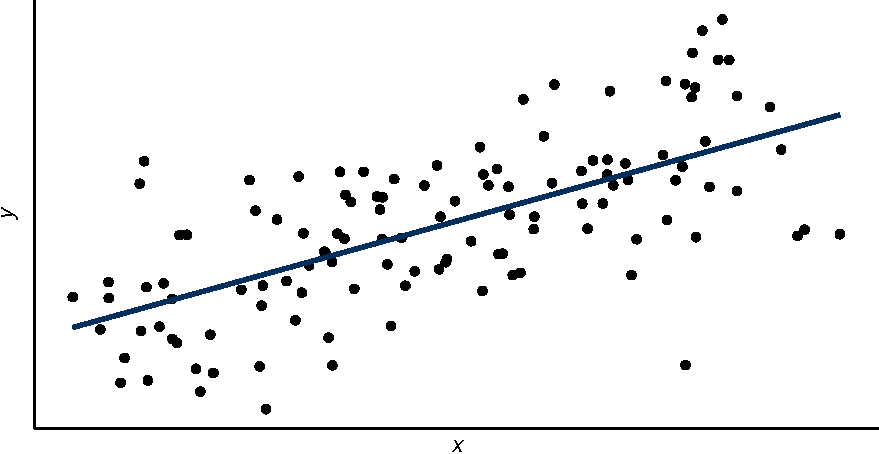
\includegraphics{figure/linear-reg-1.pdf}
\end{frame}

\begin{frame}{Varying intercepts/slopes model}
\protect\hypertarget{varying-interceptsslopes-model}{}
Suppose each unit \(i=1,\dots,n\) relates to the \(k\)th observation in
group \(j\in\{1,\dots,m\}\). Model the function \(f\) additively:
\only<1>{
$$
f(x_{kj}, j) = f_1(x_{kj}) + f_2(j) + f_{12}(x_{kj},j).
\phantom{\myunderbrace{x_{kj}^\top\beta_1}{f_1}}
$$
} \only<2>{
$$
f(x_{kj}, j) = 
\myunderbrace{x_{kj}^\top\beta_1}{f_1} + 
\myunderbrace{\beta_{0j}}{f_2} + 
\myunderbrace{x_{kj}^\top\beta_{1j}}{f_{12}}
\phantom{f_1(x_{kj})}
$$
} \vspace{-0.5em}

\begin{onlyenv}<1>
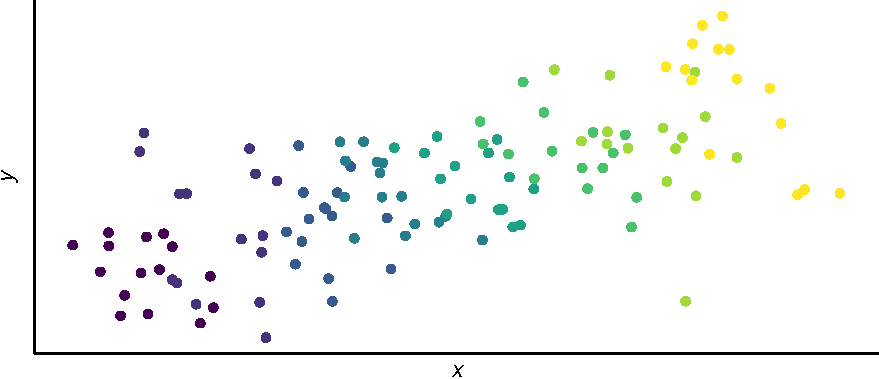
\includegraphics{figure/var-int-slope1-1.pdf}

\end{onlyenv}

\begin{onlyenv}<2>
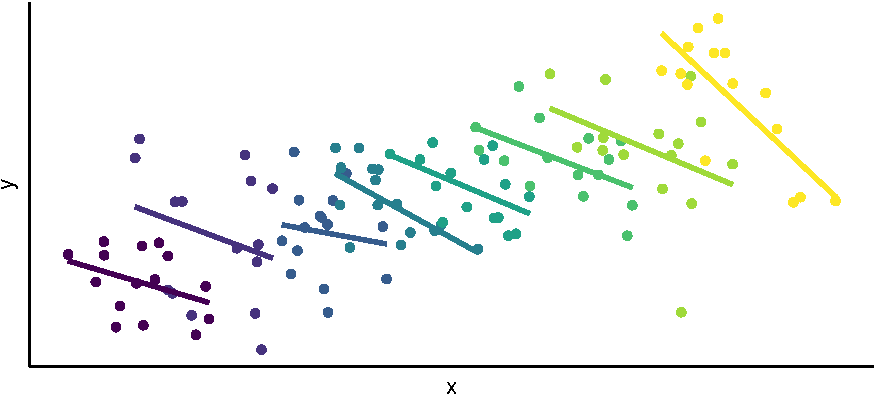
\includegraphics{figure/var-int-slope2-1.pdf}

\end{onlyenv}
\end{frame}

\begin{frame}{Smoothing models}
\protect\hypertarget{smoothing-models}{}
Suppose \(f\in\cF\) where \(\cF\) is a space of ``smoothing functions''
(models like LOESS, kernel regression, smoothing splines, etc.).

\vspace{1em}

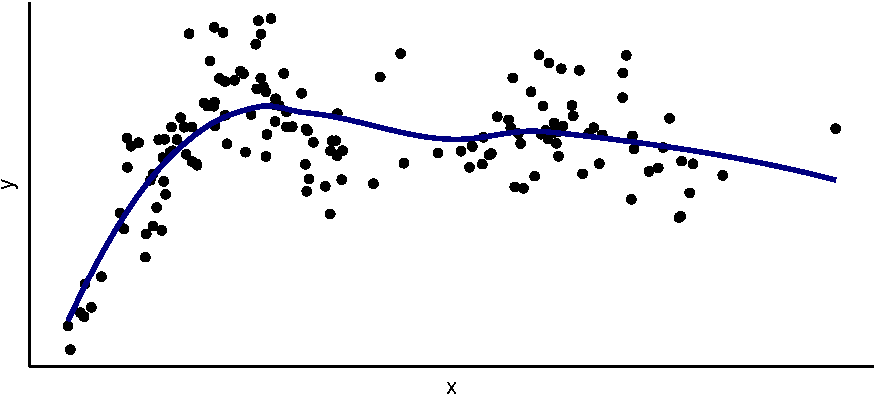
\includegraphics{figure/smooth1-1.pdf}
\end{frame}

\begin{frame}{Functional regression}
\protect\hypertarget{functional-regression}{}
Suppose the input set \(\cX\) is functional. The (linear) regression
aims to estimate a coefficient function \(\beta:\cT\to\bbR\) \[
y_i = \myunderbrace{\int_\cT x_i(t)\beta(t) \dint t}{f(x_i)} + \epsilon_i
\]

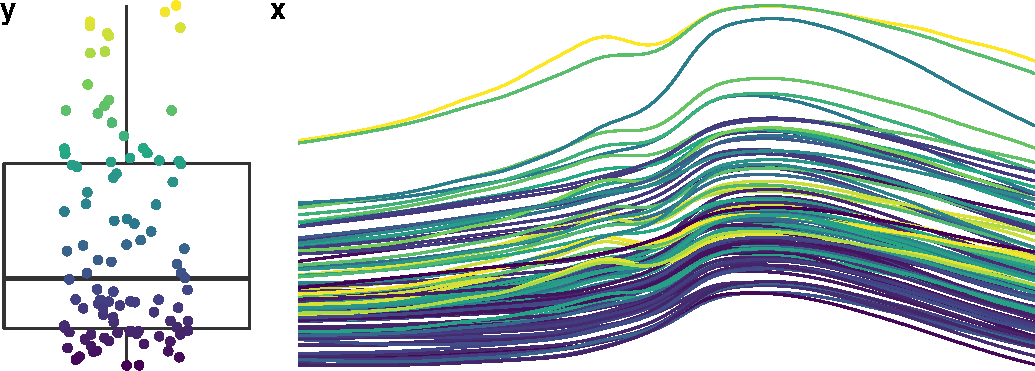
\includegraphics{figure/functionalx-1.pdf}
\end{frame}

\begin{frame}{The I-prior}
\protect\hypertarget{the-i-prior}{}
For the regression model stated in \eqref{mod1}, we assume that \(f\)
lies in some RKHS of functions \(\cF\), with reproducing kernel \(h\)
over \(\cX\).

\begin{definition}[I-prior]
\label{def:iprior} The entropy maximising prior distribution for \(f\),
subject to constraints, is \vspace{-0.7em} \begin{equation}
\begin{gathered}\label{iprior}
f(x) = \sum_{i=1}^n h(x,x_i)w_i \\
(w_1,\dots,w_n)^\top \sim \N_n(0, \Psi) \vspace{-0.7em}
\end{gathered}
\end{equation}
\end{definition}

Therefore, the covariance kernel of
\(\mathbf f = \big(f(x_1),\dots, f(x_n) \big)^\top\) is determined by
the function \vspace{-0.4em} \[
k(x,x') = \sum_{i=1}^n\sum_{j=1}^n \Psi_{i,j} h(x,x_i )h(x',x_j),
\] which happens to be \textbf{Fisher information} between two linear
forms of \(f\).
\end{frame}

\begin{frame}{The I-prior (cont.)}
\protect\hypertarget{the-i-prior-cont.}{}
Interpretation:

\vspace{-1em}

\begin{empheq}[box=\tcbhighmath]{align*}
\begin{split}
&\color{navyblue}\text{The more information about } f, \text{ the larger its prior variance,} \\[-0.2em]
&\color{navyblue}\text{and hence the smaller the influence of the prior mean (and} \\[-0.2em]
&\color{navyblue}\text{vice versa).}
\end{split}
\end{empheq}

\pause

\vspace{0.2em}

Of interest then are

\begin{enumerate}
\item
  Posterior distribution for the regression function, \[
  p(\mathbf f \,|\, \mathbf y) =
  \frac{p(\mathbf y \,|\, \mathbf f)p(\mathbf f)}
  {\int p(\mathbf y \,|\, \mathbf f)p(\mathbf f) \dint \mathbf f}.
  \]
\item
  Posterior predictive distribution (given a new data point \(x_{new}\))
  \[
  p(y_{new} \,|\, \mathbf y) = \int p( y_{new} \,|\, f_{new}) p( f_{new} \,|\, \mathbf y) \dint f_{new},
  \] where \(f_{new} = f(x_{new})\).
\end{enumerate}
\end{frame}

\begin{frame}{Introduction (cont.)}
\protect\hypertarget{introduction-cont.}{}
Observations
\(\{(y_i,x_i) \mid y_i,x_i\in\bbR \ \forall i=1,\dots,n\}\).

\vspace{1em }

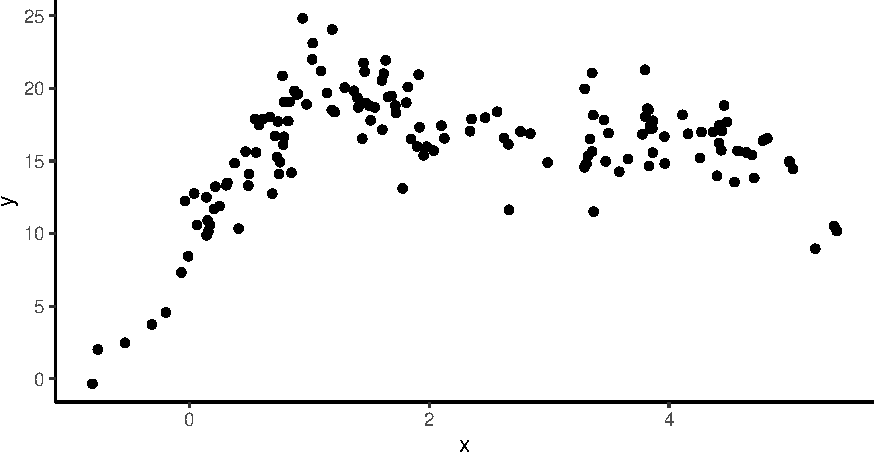
\includegraphics{figure/datapoints-1.pdf}
\end{frame}

\begin{frame}{Introduction (cont.)}
\protect\hypertarget{introduction-cont.-1}{}
Choose \(h(x,x') = e^{-\frac{\lVert x - x' \rVert^2}{2l^2}}\) (Gaussian
kernel). Sample paths from the I-prior:

\vspace{1em}

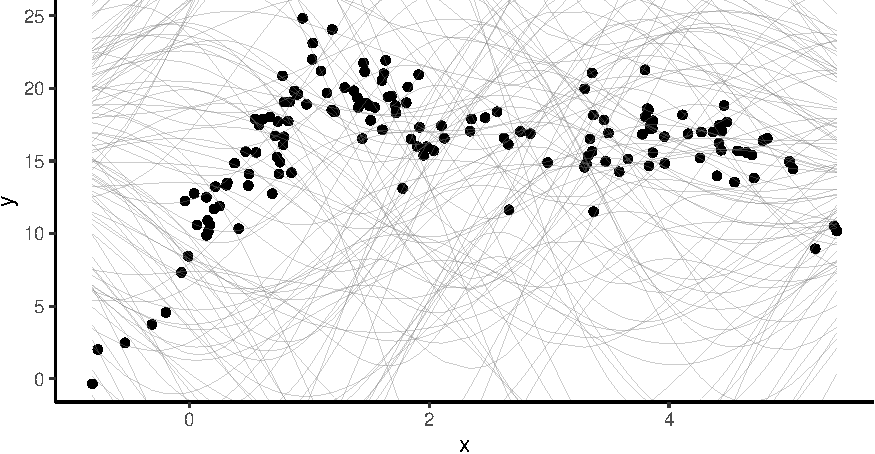
\includegraphics{figure/priorsamp-1.pdf}
\end{frame}

\begin{frame}{Introduction (cont.)}
\protect\hypertarget{introduction-cont.-2}{}
Sample paths from the posterior of \(f\):

\vspace{1em}

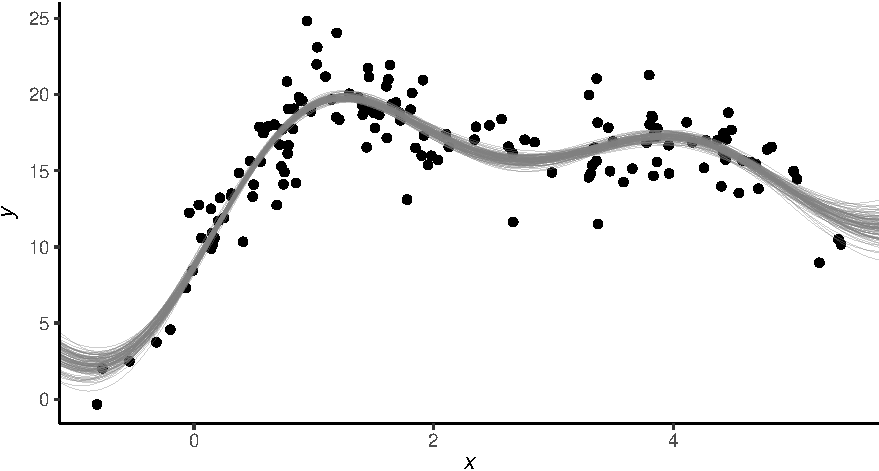
\includegraphics{figure/postsamp-1.pdf}
\end{frame}

\begin{frame}{Introduction (cont.)}
\protect\hypertarget{introduction-cont.-3}{}
Posterior mean estimate for \(y=f(x)\) and its 95\% credibility
interval.

\vspace{1em}

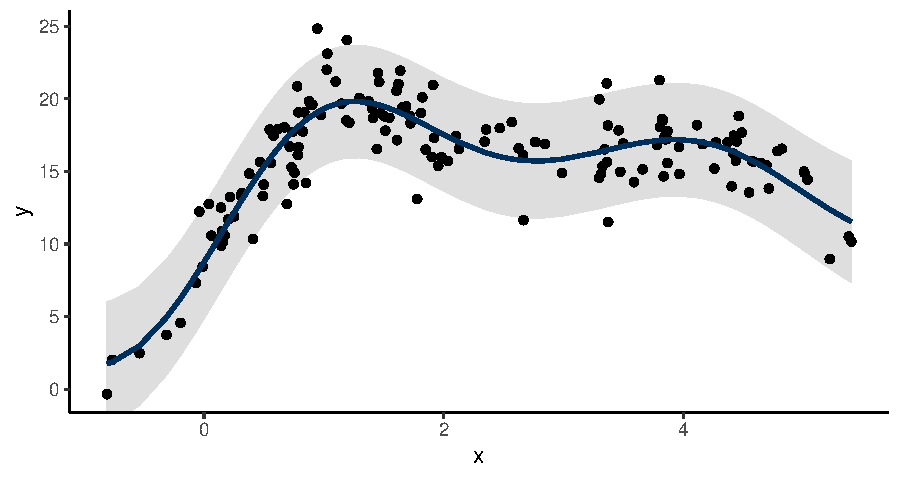
\includegraphics{figure/ipriorplot-1.pdf}
\end{frame}

\begin{frame}{Why I-priors?}
\protect\hypertarget{why-i-priors}{}
\begin{columns}[T]
\begin{column}{0.48\textwidth}
Advantages

\begin{itemize}
\item
  Provides a unifying methodology for regression.
\item
  Simple and parsimonious model specification and estimation.
\item
  Often yield comparable (or better) predictions than competing ML
  algorithms.
\end{itemize}
\end{column}

\begin{column}{0.48\textwidth}

\includegraphics[width=0.9\linewidth]{figure/wordcloud}
\end{column}
\end{columns}

Competitors:

\begin{itemize}
\item
  Tikhonov regulariser (e.g.~cubic spline smoother) \[
  \hat f = \argmin_f \sum_{i=1}^n (y_i - f(x_i))^2 + \lambda \int f''(x)^2 \dint x
  \]
\item
  Gaussian process regression
\end{itemize}
\end{frame}

\hypertarget{regression-using-i-priors}{%
\section{Regression using I-priors}\label{regression-using-i-priors}}

\hypertarget{reproducing-kernel-hilbert-spaces}{%
\subsection{Reproducing kernel Hilbert
spaces}\label{reproducing-kernel-hilbert-spaces}}

\hypertarget{the-fisher-information}{%
\subsection{The Fisher information}\label{the-fisher-information}}

\begin{frame}{The Fisher information}
Suppose further that \(f\in\cF\) where \(\cF\) is a reproducing kernel
Hilbert space (RKHS) with reproducing kernel \(h:\cX\times\cX\to\bbR\).
Then \eqref{mod1} can be expressed as \begin{equation}\label{mod2}
\begin{gathered}
y_i = \big\langle f, h(\cdot,x_i)\big\rangle_\cF + \epsilon_i \\
(\epsilon_1,\dots,\epsilon_n)^\top \sim \N(\bzero, \bPsi^{-1})
\end{gathered}
\end{equation}

The Fisher information for \(f\) is given by \[
\cI_f = \sum_{i=1}^n\sum_{j=1}^n \psi_{ij}h(\cdot,x_i) \otimes h(\cdot,x_j)
\]

It's helpful to think of \(\cI_f\) as a bilinear form
\(\cI_f:\cF \times \cF \to \bbR\) defined by \[
\cI_f = -\E\nabla^2 L(f|y)
\] so between two linear functionals of f\ldots.
\end{frame}

\begin{frame}{}
\protect\hypertarget{section}{}
where each \(y_i\in\bbR\),, and \(f\in\cF\) a reproducing kernel Hilbert
space (RKHS) with kernel \(h:\cX\times\cX\to\bbR\). The I-prior
\autocite{bergsma2019} for the regression function \(f\) is the random
function defined \begin{equation}
\begin{gathered}
f(x_i) = f_0(x_i) + \sum_{k=1}^n h(x_i,x_k)w_k \\
(w_1,\dots,w_n)^\top \sim \N(\bzero, \bPsi)
\end{gathered}
\end{equation} where \(f_0\) is some prior mean for the regression
function.
\end{frame}

\hypertarget{estimation}{%
\section{Estimation}\label{estimation}}

\hypertarget{examples}{%
\section{Examples}\label{examples}}

\hypertarget{further-research}{%
\section{Further research}\label{further-research}}

\begin{frame}{Further research}
Hello
\end{frame}




\end{document}		